\documentclass{article}
\usepackage{fontspec}
\pagestyle{empty}
\usepackage{geometry}
\geometry{paperwidth=65mm, paperheight=80mm, left=2mm, top=0mm, right=2mm, bottom=0mm}
\parindent=0pt
\usepackage{color}
\usepackage{xcolor}
\usepackage{tikz}

\begin{document}
\centering
% \vspace*{\fill} \vspace*{-15ex}

x, y:\\
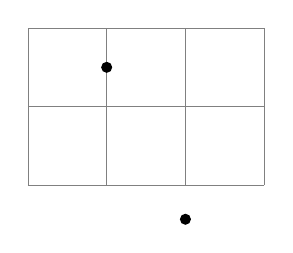
\begin{tikzpicture}
    \draw[help lines] (0,0) grid (3,2);
    \fill (1cm,1.5cm) circle (2pt);
    \fill (2cm,-5mm+2pt) circle (2pt);
\end{tikzpicture}

x, y, z:\\
\begin{tikzpicture}[->]
    \draw (0,0) -- (1,0);
    \draw (0,0) -- (0,1,0);
    \draw (0,0) -- (0,0,1);
\end{tikzpicture}

polar:\\
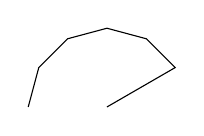
\begin{tikzpicture}
    \draw (0cm,0cm) -- (30:1cm) -- (60:1cm) -- (90:1cm)
    -- (120:1cm) -- (150:1cm) -- (180:1cm);
\end{tikzpicture}

\vspace*{\fill} 
\end{document}